\documentclass[11pt]{article}
\usepackage[a4paper,margin=2.2cm]{geometry}
\usepackage{graphicx,booktabs,amsmath,amssymb,xcolor,caption,tabularx,array,enumitem,adjustbox,multirow}
\usepackage[hidelinks]{hyperref}
\usepackage{mathptmx}
\captionsetup{font=small,labelfont=bf}
\setlength{\parskip}{3pt}
\newcolumntype{Y}{>{\raggedright\arraybackslash}X}
\newenvironment{revcomment}{\begin{quote}\itshape}{\end{quote}}
\newcommand{\answerhead}[1]{\par\medskip\noindent\textbf{#1}\par}
\title{\vspace{-1.4cm}McQueenGuard: Learning-Assisted Verification Framework for Runtime Safety Assurance of Self-Driving Systems (JSA-D-26-01243)\\[4pt]
\large Responses and additional experiments for Reviewer~\#1 (Comments~6 and 7) and Reviewer~\#2 (Comments~6 and 7)}
\date{}
\begin{document}
\maketitle
\vspace{-1.3cm}
\noindent This document contains (Part~I) the answers to the four comments for the revision letter and (Part~II) the new
material for Section~6 of the manuscript. The comparison, ablation and out-of-distribution analyses (Sections~6.9--6.11) share one set of experiments: all methods
and ablation variants were run on the same 600 scenario instances. The embedded-timing and sensor-noise shift experiments of
Section~6.12 are separate runs with the same scenario generator.
Table and figure numbers continue the numbering of the manuscript (the last table in Section~6 is Table~5 and the last figure is
Figure~17); the comparison table of Section~7 (currently Table~6) becomes Table~19.

\tableofcontents

%=====================================================================================================
\part*{Part I \quad Answers for the revision letter}
\addcontentsline{toc}{part}{Part I \quad Answers for the revision letter}

\section*{Reviewer \#1, Comment 6}
\addcontentsline{toc}{section}{Reviewer \#1, Comment 6}
\begin{revcomment}
``Could you supplement the desktop-based experiments with latency, memory footprint, and power consumption data when deploying
the MLP verifier on an automotive-grade embedded platform (e.g., NVIDIA Orin)? How would the framework handle domain adaptation
challenges, such as simulation-to-real shifts in sensor noise distributions, to substantiate claims of embedded system
applicability?''
\end{revcomment}
\answerhead{Answer:}
We thank the reviewer for this suggestion. We have added a deployment study and a sensor-noise shift study to the revised
manuscript (please see the new Section~6.12, Tables~\ref{tab:emb}--\ref{tab:sc} and Figures~\ref{fig:et}--\ref{fig:ss}).

\emph{Embedded profile.} The learned verifier has 7,786 parameters (30\,KiB in
FP32, 14\,KiB as an INT8 ONNX model) and needs 7,616 multiply-accumulate
operations per inference. On one CPU thread, MLP inference takes 8.3\,$\mu$s with ONNX Runtime and
a complete learned decision (feature extraction, inference, familiarity check, admission test and action selection) takes
43.6\,$\mu$s on average (94.6\,$\mu$s at the 99th percentile), compared with 392\,ms for exact
verification with PRISM. A minimal inference process occupies 54\,MB of resident memory,
of which the inference session accounts for 9\,MB; the PRISM verification
server occupies up to 251\,MB. We did not have access to an NVIDIA Orin board during the
revision. We therefore report projected latencies for the Arm Cortex-A78AE CPU of the Jetson AGX Orin under an explicit
1.5--4$\times$ single-thread slow-down band, and an upper bound on the energy per decision derived from the 15--60\,W module
power envelope (1.6--6.5\,mJ for a
learned decision versus 15--59\,J for an exact
verification at the central slow-down). These are projections, not measurements, and we state this in the manuscript. To check
whether the closed-loop results survive slower hardware, we re-ran 100 paired episodes with every computation time
multiplied by 2.5. The learned decision path remained far below the 100\,ms decision period, but McQueenGuard's safety
violations rose from 5\,\% to 7\,\%
(2 more of 100 episodes, an indicative rather than significant
difference), consistent with each fallback waiting longer for PRISM. On an embedded platform the exact verifier is therefore the bottleneck, and we
discuss running it on a dedicated core with a bounded model size.

\emph{Sensor-noise shift.} We evaluated an unannounced shift of the perception noise model (heavy-tailed noise, a systematic
bias, additional drop-outs and latency, at three severity levels). Three mechanisms of the framework act under such a shift:
the familiarity check routes unfamiliar inputs to exact verification; the exact results of these fallbacks are fed back to
recalibrate the error margin over a rolling window (Algorithm~1, lines~27--28), complemented by shadow audits of 10\,\% of the
admitted decisions; and the Simplex shield remains active independently of the learned verifier. Under the shift the
coverage of the offline margin varied between 92.9 and 95.4\,\%
(94.1\,\% at the highest severity), and the unsafe-admission rate of the static margin rose from 2.2\,\% to
3.8\,\% of admitted decisions. With recalibration the margin grew from
0.018 to 0.033 and the unsafe-admission rate remained between
1.1 and 1.8\,\% across the severities, at the cost of admitting fewer decisions
(67\,\% instead of 79\,\%).
Recalibration does not restore exchangeability, so under a persistent shift the statistical statement remains conditional on the
recalibration window; we state this in Section~6.13 and list on-vehicle validation as future work. The ONNX models and the
benchmarking scripts are included in the project repository so that the measurements can be repeated on the target hardware.

\section*{Reviewer \#1, Comment 7}
\addcontentsline{toc}{section}{Reviewer \#1, Comment 7}
\begin{revcomment}
``Could you expand the baseline comparisons to include (1) other learning-assisted verification frameworks (e.g., VerifAI),
(2) conventional autonomous driving planners (e.g., MPC, rule-based methods), and (3) end-to-end reinforcement learning planners
to better highlight McQueenGuard's advantages in safety assurance and real-time efficiency?''
\end{revcomment}
\answerhead{Answer:}
We thank the reviewer for this suggestion. We have added a closed-loop comparison (please see the new Sections~6.8 and 6.9,
Tables~\ref{tab:methods}--\ref{tab:c7b} and Figures~\ref{fig:c7a}--\ref{fig:c7c}) with (1) a VerifAI-based runtime-assurance
pipeline (falsification with VerifAI's cross-entropy sampler, a learned violation monitor and Simplex switching to a braking
controller), (2) the collision-avoidance MPC of Zhang et al.\ (IEEE T-ITS, 2022) and a rule-based planner (Intelligent Driver
Model with emergency braking), and (3) an end-to-end PPO planner trained with a CaRL-style reward. McQueenGuard with exact
verification at every decision is included as a reference. All methods ran on the same 600 scenario instances (60
per scenario category of Table~3). McQueenGuard had a collision rate of 1.0\,\% and a safety-violation rate
(collision or violation of the 2\,m safe margin) of 4.8\,\%, compared with
3.5\,\% for VerifAI, 9.0\,\% for MPC, 6.0\,\%
for the rule-based planner and 8.0\,\% for end-to-end PPO. In paired McNemar tests McQueenGuard had significantly fewer safety violations than MPC and end-to-end PPO ($p<0.001$, $p=0.014$); the differences to the rule-based planner and VerifAI were not significant ($p=0.32$, $p=0.22$). Its collision rate was the lowest of the six methods in Table~\ref{tab:c7} and significantly lower than that of MPC and the rule-based planner ($p<0.001$, $p=0.002$). The share of executed control commands whose exactly verified unsafe probability was at least $\theta$ was 14.4\,\% for McQueenGuard, lower than for MPC, the rule-based planner and end-to-end PPO (18.0--21.8\,\%) and higher than for VerifAI (12.6\,\%). McQueenGuard is the only method that attaches a
calibrated error bound to each admitted decision. With respect to
real-time efficiency, 86\,\% of McQueenGuard's decisions were taken by the learned verifier in
microseconds, which reduced the mean decision latency from 334\,ms (exact verification at every
decision) to 49\,ms and the share of decisions missing the 100\,ms decision period from
93\,\% to 13\,\%. The comparison also shows the costs of the approach, which we
report in the manuscript: McQueenGuard is more cautious than MPC and the rule-based planner (median travel-time ratio
1.64 against 1.38 and 1.37), the remaining
violations occur mainly while a fallback waits for PRISM and in the novel-trajectory category, whose occluded and running
pedestrians are not represented in the verification model, and VerifAI reached a similar violation rate but deadlocked in
20.8\,\% of the episodes.

\section*{Reviewer \#2, Comment 6}
\addcontentsline{toc}{section}{Reviewer \#2, Comment 6}
\begin{revcomment}
``The experimental evaluation demonstrates substantial latency reduction and relatively small approximation errors, but it could
be strengthened in two aspects. First, an ablation study is needed to distinguish the contribution of the learned verifier from
that of the proposed error-aware admission and exact fallback mechanisms. The evaluation should also provide larger-scale
evidence on decision preservation and safety outcomes rather than relying mainly on illustrative cases.''
\end{revcomment}
\answerhead{Answer:}
We thank the reviewer for this valuable comment. We have added an ablation study and a large-scale preservation analysis
(please see the new Section~6.10, Tables~\ref{tab:abl}--\ref{tab:th1} and Figures~\ref{fig:abl}--\ref{fig:pres}).

\emph{Ablation.} Starting from the complete framework, we removed one component at a time: the conformal margin, the
familiarity check, the exact fallback (replaced by the conservative fallback control), the whole admission mechanism (learned
verifier only), the Simplex shield, and the learned verifier itself (exact verification only). Each variant ran on the same
600 scenario instances (5,400 closed-loop runs in total, including the idealised reference described below). The results separate the
contributions as follows. The learned verifier is what makes runtime verification feasible: with exact verification at every
decision, 93\,\% of the decisions missed the 100\,ms decision period and the safety-violation rate was
9.3\,\% (4.8\,\% for the complete framework). The error-aware admission
controls how often a learned result is wrongly admitted: on the exactly verified decision stream, the share of decisions in
which an action with exact unsafe probability $\ge\theta$ was admitted fell from 5.36\,\% to
1.99\,\% in-distribution and from 12.15\,\% to
0.77\,\% out of distribution, and in closed loop the margin reduced the share of executed
commands with verified risk above $\theta$ from 21.4\,\% to 14.4\,\%.
The exact fallback is what keeps the vehicle making progress when the learned verifier is not admitted: replacing it by the
conservative fallback control gave the lowest violation rate (1.0\,\%) but
24.7\,\% deadlocks, including every episode of the high-noise and unseen-weather categories. Removing the
Simplex shield raised the safety-violation rate to 14.8\,\% ($p<0.001$),
because the shield covers the interval in which an exact result is pending. The deployable variants with fewer violations than the complete
framework either deadlocked more often or had no bound on false admissions, so no single component can be removed without losing
liveness, safety or the statistical guarantee. An idealised reference in which exact results are available without delay reached 1.7\,\% safety violations and 0.0\,\% deadlocks, which locates the remaining gap of the complete framework in the latency of the exact fallback rather than in the admission logic.

\emph{Larger-scale preservation evidence.} Instead of the twelve illustrative cases of Table~2, every third decision of the
complete framework in all 600 episodes was additionally verified exactly for all candidate actions
(25,466 decisions). Safety preservation holds at this scale within the stated statistical bound: false admissions
occurred in 1.69\,\% of all decisions and in at most 3.34\,\% in any
scenario category, below $\alpha=5\,\%$ (Corollary~1). Decision preservation in the sense of Theorem~1 is more limited: the admitted
learned decision coincided with the exact decision in 60.3\,\% of the cases. Where it differed, the
learned action was safe in 96\,\% of the cases and more cautious than the
exact action in 69\,\%, and the mean utility loss was
0.016 (utilities range from 0 to about 1.3). The sufficient condition of Theorem~1 was
verified at scale (whenever the realised utility error satisfied $2\max_a|U(a)-\hat U(a)|<\mathcal{T}(k)$, the decisions agreed in
100.0\,\% of 690 cases), but with the calibrated utility margin
($\varepsilon_U=0.101$) it was not satisfied by any decision, because the utility gap between the best and second-best admissible actions is small (median 0.007).
We have therefore qualified the claims about decision preservation in Sections~5.1, 6.5 and 6.10: the guarantee that matters for
safety is the admission bound, whereas exact agreement of the selected action is not guaranteed in general.

\section*{Reviewer \#2, Comment 7}
\addcontentsline{toc}{section}{Reviewer \#2, Comment 7}
\begin{revcomment}
``Second, the reported empirical error-bound coverage (97.8\%) does not by itself demonstrate that the estimated bound remains
reliable for unknown or out-of-distribution scenarios. The authors should evaluate the error-bound coverage and false-admission
rate under OOD conditions, together with the resulting fallback and safety outcomes. Finally, the reported latency improvement
should clarify whether it represents end-to-end runtime overhead or only learned-model inference time.''
\end{revcomment}
\answerhead{Answer:}
We agree with the reviewer and thank them for this comment. We have added an out-of-distribution evaluation of the error bound
and a latency breakdown (please see the new Section~6.11, Tables~\ref{tab:ood}--\ref{tab:lat} and Figure~\ref{fig:ood}), and we
have extended the sensor-noise shift study of Section~6.12. The learned verifier was trained and calibrated only on the six
in-distribution categories of Table~3; the high-speed, novel-trajectory, high-noise and unseen-weather (snow) categories are out
of distribution. For each category we report the coverage of the calibrated margin, the false-admission rate, the fallback rate
and the closed-loop safety outcomes, all on the decisions taken by the framework itself. The results show that an in-distribution coverage
figure, such as the 97.8\,\% of Table~4 (obtained for the CARLA verifier; our testbed verifier has 94.5\,\%), does not by itself carry over to
shifted conditions:
\begin{itemize}[leftmargin=1.3em,itemsep=1pt]
\item In-distribution, the coverage of the margin over all decisions was 94.5--96.9\,\%,
consistent with the nominal 95\,\%. On the subset of risk-relevant decisions it was lower
(86.8--93.0\,\%), which illustrates that the conformal guarantee is
marginal rather than conditional. False admissions remained at or below 3.34\,\% of the decisions.
\item Out of distribution, coverage depends on the type of shift. Under unseen weather it fell to 89.6\,\%
(82.2\,\% on risk-relevant decisions), i.e., the margin is not reliable there. The familiarity check
rejected all high-noise and unseen-weather decisions (fallback rate 100\,\%), so no learned result was admitted in these categories;
without the check, 5.61\,\% of the unseen-weather decisions would have been false admissions, and
28.60\,\% without any admission rule. At high speed the fallback rate rose to 21.0\,\% and false admissions stayed at
2.18\,\%. Novel trajectories were not detected as unfamiliar
(98.5\,\% familiar) and the margin remained valid there (97.9\,\% coverage),
but this category had the highest safety-violation rate of the complete framework (18.3\,\%), and exact
verification only reached the same level (18.3\,\%). These violations come from the verification model, which does
not represent occluded or running pedestrians, and not from the learned approximation; the admission rule cannot detect them, and we
now state this limitation explicitly. In the high-speed, high-noise and unseen-weather categories, the remaining violations
(10.0, 6.7 and 6.7\,\%, i.e. 6, 4 and 4 of 60 episodes) did not occur when exact
results were made available without delay, which points to the latency of the exact fallback as their cause (significant for the high-speed category,
indicative for the other two).
\item The familiarity check detects shifts of the input distribution (sensor noise, friction outside the training range) but is a
weak predictor of individual bound failures (area under the ROC curve 0.56). It complements, but does not replace,
the online recalibration described in our answer to Reviewer~\#1, Comment~6.
\end{itemize}
\emph{Latency.} The speed-up reported in Table~4 (2.1\,ms against 148.6\,ms) compares the inference time of the learned verifier
with the time of one exact PRISM verification; it is not the end-to-end runtime overhead. We have relabelled these rows and added a
breakdown (Table~\ref{tab:lat}). In our measurements, MLP inference takes 8.3\,$\mu$s, a complete
learned decision 43.6\,$\mu$s and an exact verification 392\,ms, of which
99\,\% is model construction and model checking inside PRISM. Because a share of decisions still falls back to
exact verification, the end-to-end reduction of the mean decision latency is 6.8$\times$
(334\,ms to 49\,ms, an 85\,\% reduction), much smaller than the
inference-only ratio; although only 14\,\% of the decisions are exact, they occupy 36\,\% of the driving time,
because each exact verification blocks the planner until it completes. Perception and actuation latencies are the same for all methods and are not included in these figures.

%=====================================================================================================
\clearpage
\part*{Part II \quad New material for Section 6 of the manuscript}
\addcontentsline{toc}{part}{Part II \quad New material for Section 6 of the manuscript}
\setcounter{table}{5}
\setcounter{figure}{17}

\section*{6.8 \quad Extended Closed-Loop Evaluation: Setup}
\addcontentsline{toc}{section}{6.8 Extended closed-loop evaluation: setup}
The experiments in Sections~6.2--6.7 study the framework in CARLA on a limited number of scenarios. To compare McQueenGuard with
alternative approaches and with its own ablations on identical scenario instances, at a scale of thousands of closed-loop runs, and
with computation latency inside the control loop, we use a reproducible closed-loop testbed that re-implements the
pedestrian-crossing scenario of Section~6.1. The testbed is not a substitute for CARLA; its purpose is a controlled, paired
comparison.

\textbf{Scenario.} The ego vehicle (length 4.7\,m) approaches a marked crosswalk from 70\,m at the scenario speed. A pedestrian waits at
the kerb and crosses with probability 0.75, at 1.0--1.8\,m/s, with a hesitation inside the lane in 30\,\% of the crossings; a
pedestrian who waits at the kerb crosses once the vehicle has stopped in front of the crosswalk. The weather presets use the friction,
camera-noise, LiDAR-accuracy and perception-latency values of the CARLA configuration of Section~6. Detection probability decays with
distance and visibility, tracks drop out, positions are measured with noise and arrive after a perception latency of 90--150\,ms, and
actuation has a 0.1\,s delay and a 0.2\,s first-order lag with friction-limited deceleration. Every planner is invoked every 100\,ms,
and its command takes effect only after its own computation time has elapsed; the previous command is held meanwhile.

\textbf{Scenario categories.} We use the ten categories of Table~3, with 60 scenario instances each (600 per method). The six
clear, fog and rain categories are in-distribution: the verified dataset of the learned verifier was collected only in these
categories. The other four are out of distribution: high speed (50--60\,km/h), novel trajectory (running pedestrians, 2.5--3.5\,m/s, or
pedestrians occluded until they step into the road), high noise (three times the measurement noise and 15\,\% additional
drop-outs) and unseen weather (snow, friction about 0.3, visibility about 32\,m).

\textbf{McQueenGuard.} At each decision point the parametric MDP is instantiated with the current valuation $\lambda$ (estimated friction,
perception-error probability, visibility, pedestrian speed, crossing intention and presence belief) and verified for five longitudinal
actions (accelerate, maintain speed, reduce speed, brake, emergency brake) against $P_{\max}{=}?[F^{\le 4\,\mathrm{s}}\,\mathit{unsafe}]$,
where \emph{unsafe} is a collision or a violation of the safe margin $d_{SM}=2$\,m, and the performance reward
$R_{\max}{=}?[C^{\le 4\,\mathrm{s}}]$, with $\theta=0.05$ and the safety-first lexicographic rule of Equations~(16)--(17). Exact
verification uses PRISM~4.8.1 (sparse engine) as a persistent verification server. The learned verifier is the MLP of Section~6.6
(18 inputs; 64, 64 and 32 hidden units), trained on 10,876 exactly verified decision points from 280 episodes
(episode-wise 70/15/15\,\% split), with an MAE of 0.0153 for the unsafe probability and 0.0259 for the utility. The
split-conformal margin of Equation~(25) at $\alpha=0.05$ is $\varepsilon=0.018$, with 94.5\,\% coverage on the
1,549 test decisions (95\,\% interval [93.3, 95.5]\,\%, consistent with the nominal 95\,\%). Because the admitted action is chosen after the estimates are computed, the calibration residual is taken simultaneously over
all candidate actions whose estimate lies below $\theta$, which makes Corollary~1 hold for whichever action is admitted. The familiarity set
$\mathcal{H}$ is implemented as a Mahalanobis-distance test (99th percentile of the calibration set) combined with the training range of every
feature. While an exact result is pending after a non-admitted decision, the fallback safety control (Algorithm~1, line~26) applies at
least the reduce-speed action, and the Simplex shield of Section~4.5 is evaluated every 50\,ms.

\textbf{Metrics.} A \emph{safety violation} is a collision or a gap below $d_{SM}=2$\,m while the pedestrian is in the lane. The \emph{verified
risk} is the share of executed control commands, audited once per second, whose exact 4-s unsafe probability is at least $\theta$; it
includes unavoidable states and is therefore not zero for any method. A \emph{deadlock} is an episode in which the vehicle does not clear the
crosswalk within 30\,s of its free-flow arrival time. The \emph{travel-time ratio} is the time needed to clear the crosswalk divided by the
free-flow time. A \emph{deadline miss} is a decision whose computation exceeds the 100\,ms decision period. Rates are given with 95\,\%
Wilson intervals, and paired differences are tested with exact McNemar tests on the same scenario instances.

\textbf{Hardware.} All timings were measured on one machine (Intel Xeon at 2.1\,GHz, single-threaded inference), which differs from the
desktop used in Sections~6.2--6.7; absolute times are therefore not directly comparable with Figure~14 and Table~4. Because computation
times are measured rather than simulated, a repeated run can differ in individual episodes when a method's computation time is close to a
timing threshold; in a re-run of 21 embedded-timing episodes for every method, all outcomes were reproduced except one MPC episode.

\begin{table}[h]
\centering\small
\caption{Methods and ablation variants evaluated in Sections~6.9 and 6.10.}\label{tab:methods}
\begin{tabularx}{\linewidth}{lY}
\toprule
Method & Description \\
\midrule
McQueenGuard & Learned verifier with error-aware admission (margin $\varepsilon$, familiarity set $\mathcal{H}$, $\varepsilon\le\varepsilon_{\max}$), exact PRISM fallback, Simplex shield \\
McQueenGuard (exact only) & Exact PRISM verification at every decision, Simplex shield \\
VerifAI runtime assurance & Scenario space and falsification with VerifAI (cross-entropy sampler, 400 falsification runs) against $\mathbf{G}(\mathit{gap}\ge d_{SM})\wedge\neg\mathit{collision}$; a decision-tree monitor learned from the traces predicts a violation within 2\,s (threshold for $\ge$95\,\% recall) and switches the PPO planner to a braking controller \\
MPC & Collision-avoidance MPC of Zhang et al.\ (2022): 4-s horizon, 0.1-s step, speed-tracking and smoothness cost, input and friction-limited deceleration bounds, constant-velocity pedestrian prediction and safe-distance constraint with reaction time; CVXPY with OSQP as in the authors' MPC-ROS code \\
Rule-based (IDM+AEB) & Intelligent Driver Model with a virtual stop line for a detected crossing pedestrian and emergency braking at a time-to-collision of 1.4\,s \\
End-to-end RL (PPO) & PPO policy (Stable-Baselines3, two layers of 128 units) from the 18 perception features and the desired speed to acceleration, trained for 2.5\,M steps in the in-distribution categories with a CaRL-style reward (progress multiplied by comfort and speed factors, termination and penalty on collision) \\
Ablation variants & One component removed from McQueenGuard at a time (Table~\ref{tab:abl}) \\
\bottomrule
\end{tabularx}
\end{table}

%-----------------------------------------------------------------------------------------------------
\section*{6.9 \quad Comparison with Alternative Approaches}
\addcontentsline{toc}{section}{6.9 Comparison with alternative approaches}
Table~\ref{tab:c7} summarises the results over all ten categories, and Table~\ref{tab:c7b} separates the in-distribution and
out-of-distribution categories. Figure~\ref{fig:c7a} shows the safety violations per scenario group, Figure~\ref{fig:c7b} the verified
risk of the executed commands and Figure~\ref{fig:c7c} the decision latency.

\begin{table}[h]
\centering\small
\caption{Closed-loop results over all ten scenario categories (600 paired episodes per method; 95\,\% interval of the
safety-violation rate in brackets).}\label{tab:c7}
\begin{adjustbox}{max width=\linewidth}
\begin{tabular}{lcccccccc}
\toprule
 & Collision & Safety violation & Verified risk & Deadlock & Travel-time & \multicolumn{2}{c}{Decision latency (ms)} & Deadline \\
Method & (\%) & (\%) & $\ge\theta$ (\%) & (\%) & ratio & mean & p99 & misses (\%) \\
\midrule
McQueenGuard & 1.0 & 4.8 [3.4, 6.9] & 14.4 & 1.5 & 1.64 & 49 & 794 & 12.9 \\
McQueenGuard (exact only) & 2.0 & 9.3 [7.3, 11.9] & 24.0 & 2.2 & 1.65 & 334 & 1,525 & 92.7 \\
VerifAI RA & 1.5 & 3.5 [2.3, 5.3] & 12.6 & 20.8 & 1.60 & 0.07 & 0.18 & 0.0 \\
MPC & 4.5 & 9.0 [7.0, 11.6] & 21.8 & 0.0 & 1.38 & 12 & 51 & 0.1 \\
Rule-based (IDM+AEB) & 3.2 & 6.0 [4.4, 8.2] & 18.0 & 0.0 & 1.37 & $<$0.01 & $<$0.01 & 0.0 \\
End-to-end RL (PPO) & 1.7 & 8.0 [6.1, 10.4] & 18.7 & 0.2 & 1.49 & 0.04 & 0.17 & 0.0 \\
\bottomrule
\end{tabular}
\end{adjustbox}
\end{table}

\begin{table}[h]
\centering\small
\caption{In-distribution (6 categories, 360 episodes) and out-of-distribution (4 categories, 240 episodes) results, in \%.}\label{tab:c7b}
\begin{tabular}{lcccccc}
\toprule
 & \multicolumn{3}{c}{In-distribution} & \multicolumn{3}{c}{Out-of-distribution} \\
\cmidrule(lr){2-4}\cmidrule(lr){5-7}
Method & Collision & Safety violation & Deadlock & Collision & Safety violation & Deadlock \\
\midrule
McQueenGuard & 0.0 & 1.1 & 1.9 & 2.5 & 10.4 & 0.8 \\
McQueenGuard (exact only) & 0.3 & 6.9 & 3.1 & 4.6 & 12.9 & 0.8 \\
VerifAI RA & 0.3 & 1.1 & 17.2 & 3.3 & 7.1 & 26.2 \\
MPC & 0.8 & 4.7 & 0.0 & 10.0 & 15.4 & 0.0 \\
Rule-based (IDM+AEB) & 0.8 & 1.9 & 0.0 & 6.7 & 12.1 & 0.0 \\
End-to-end RL (PPO) & 0.8 & 5.6 & 0.0 & 2.9 & 11.7 & 0.4 \\
\bottomrule
\end{tabular}
\end{table}

\begin{figure}[h]
\centering
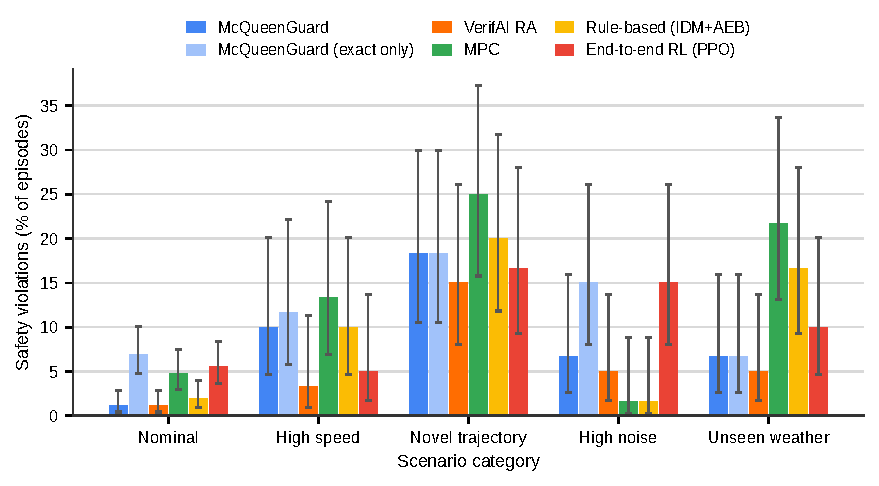
\includegraphics[width=0.92\linewidth]{../figures/fig_c7_safety_by_group.pdf}
\caption{Safety violations (collision or safe-margin violation) per scenario group, with 95\,\% Wilson intervals.}\label{fig:c7a}
\end{figure}
\begin{figure}[h]
\centering
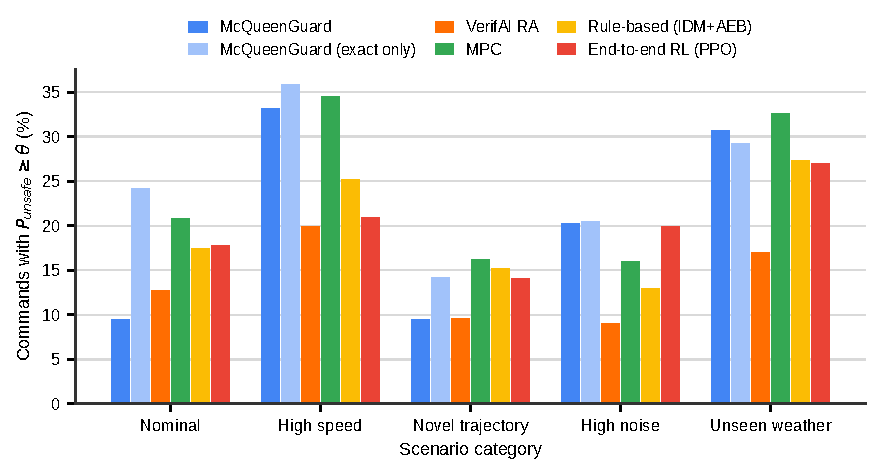
\includegraphics[width=0.92\linewidth]{../figures/fig_c7_risk.pdf}
\caption{Share of audited control commands whose exactly verified 4-s unsafe probability is at least $\theta=0.05$.}\label{fig:c7b}
\end{figure}
\begin{figure}[h]
\centering
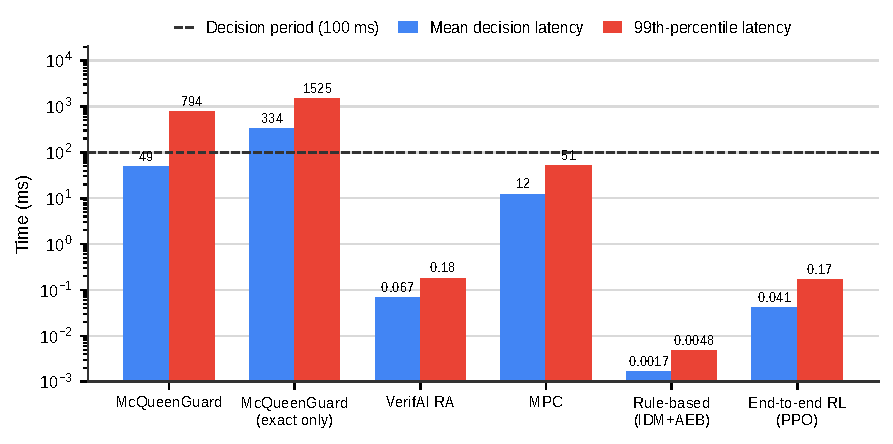
\includegraphics[width=0.92\linewidth]{../figures/fig_c7_latency.pdf}
\caption{Decision latency per method (log scale). McQueenGuard's values include the decisions that fall back to PRISM; a learned
decision alone takes 43.6\,$\mu$s on average (Table~\ref{tab:lat}).}\label{fig:c7c}
\end{figure}

\textbf{Findings.}
\begin{itemize}[leftmargin=1.3em,itemsep=2pt]
\item \emph{Safety.} McQueenGuard had 1.0\,\% collisions and 4.8\,\% safety violations. In paired McNemar tests McQueenGuard had significantly fewer safety violations than MPC and end-to-end PPO ($p<0.001$, $p=0.014$); the differences to the rule-based planner and VerifAI were not significant ($p=0.32$, $p=0.22$). The three significant differences remain significant after Holm correction for the five comparisons. Its collision rate was the lowest of the six methods in Table~\ref{tab:c7} and significantly lower than that of MPC and the rule-based planner ($p<0.001$, $p=0.002$).
\item \emph{In and out of distribution.} In-distribution, McQueenGuard had 0.0\,\% collisions and 1.1\,\% safety violations. Out of distribution all methods degraded; McQueenGuard reached 10.4\,\%, against 15.4\,\% for MPC, 12.1\,\% for the rule-based planner, 11.7\,\% for PPO and 7.1\,\% for VerifAI. 11 of its 25 out-of-distribution violations occurred in the novel-trajectory category, the rest while exact fallbacks were pending (Sections~6.10 and 6.11).
\item \emph{Assurance of the executed commands.} The share of executed control commands whose exactly verified unsafe probability was at least $\theta$ was 14.4\,\% for McQueenGuard, lower than for MPC, the rule-based planner and end-to-end PPO (18.0--21.8\,\%) and higher than for VerifAI (12.6\,\%). The verified risk includes unavoidable states; for McQueenGuard it falls to 9.1\,\% when exact results are available without delay (Section~6.10), so part of it is caused by the latency of the exact fallback. Only McQueenGuard attaches a calibrated bound to each admitted decision.
\item \emph{Real-time efficiency.} Exact verification at every decision (334\,ms mean, 1,525\,ms at the 99th percentile) missed the decision period in 93\,\% of the decisions and reacted late, which explains its 9.3\,\% safety violations although every decision was verified. McQueenGuard took 86\,\% of its decisions with the learned verifier and missed the decision period in 13\,\% of the decisions, all of them exact fallbacks. MPC needed 12\,ms per decision; the rule-based planner, PPO and VerifAI need less than 1\,ms.
\item \emph{Costs.} McQueenGuard is more cautious than MPC and the rule-based planner (median travel-time ratio 1.64 against 1.38 and 1.37) and deadlocked in 1.5\,\% of the episodes. VerifAI reached a similar violation rate (3.5\,\%) but deadlocked in 20.8\,\% of the episodes, because its monitor keeps the braking controller engaged once a violation is predicted.
\end{itemize}

%-----------------------------------------------------------------------------------------------------
\clearpage
\section*{6.10 \quad Ablation Study and Large-Scale Preservation Analysis}
\addcontentsline{toc}{section}{6.10 Ablation study and large-scale preservation analysis}
\textbf{Ablation.} Table~\ref{tab:abl} and Figure~\ref{fig:abl} report the complete framework, seven reduced variants and an idealised reference
on the same 600 scenario instances. Each reduced variant removes one component (the variant ``learned verifier only, $-$ Simplex shield''
removes the admission mechanism, the exact fallback and the shield).

\begin{table}[h]
\centering\small
\caption{Ablation study (600 paired episodes per variant). $p$: exact McNemar test of the safety-violation rate against the complete
framework (all $p<0.05$ remain below 0.05 after Holm correction for the eight comparisons). Decision modes: share of decisions taken by the learned verifier / by exact verification / by the conservative fallback control.}\label{tab:abl}
\begin{adjustbox}{max width=\linewidth}
\begin{tabular}{lccccccccccc}
\toprule
 & Collision & \multicolumn{4}{c}{Safety violation (\%)} & Deadlock & Travel-time & Verified risk & Decision modes & Latency & Deadline \\
\cmidrule(lr){3-6}
Variant & (\%) & all & $p$ & ID & OOD & (\%) & ratio & $\ge\theta$ (\%) & (\%) & mean (ms) & misses (\%) \\
\midrule
Full McQueenGuard & 1.0 & 4.8 & -- & 1.1 & 10.4 & 1.5 & 1.64 & 14.4 & 86 / 14 / 0 & 49 & 12.9 \\
$-$ conformal margin ($\varepsilon{=}0$) & 1.5 & 5.2 & $p=0.88$ & 2.8 & 8.8 & 0.3 & 1.62 & 21.4 & 86 / 14 / 0 & 48 & 12.9 \\
$-$ familiarity gate $\mathcal{H}$ & 1.0 & 2.0 & $p<0.001$ & 0.6 & 4.2 & 8.5 & 1.68 & 8.6 & 96 / 4 / 0 & 16 & 4.0 \\
$-$ exact fallback$^{a}$ & 0.3 & 1.0 & $p<0.001$ & 0.0 & 2.5 & 24.7 & 1.67 & 2.5 & 53 / 0 / 47 & 0.05 & 0.0 \\
Learned verifier only$^{b}$ & 0.8 & 1.5 & $p<0.001$ & 0.3 & 3.3 & 6.7 & 1.63 & 14.3 & 100 / 0 / 0 & 0.07 & 0.0 \\
$-$ Simplex shield & 7.0 & 14.8 & $p<0.001$ & 5.3 & 29.2 & 1.0 & 1.60 & 14.2 & 86 / 14 / 0 & 47 & 12.7 \\
Learned verifier only, $-$ Simplex shield & 0.8 & 2.7 & $p=0.024$ & 1.4 & 4.6 & 6.7 & 1.63 & 14.3 & 100 / 0 / 0 & 0.05 & 0.0 \\
Exact verification only$^{c}$ & 2.0 & 9.3 & $p<0.001$ & 6.9 & 12.9 & 2.2 & 1.65 & 24.0 & 0 / 100 / 0 & 334 & 92.7 \\
\midrule
Full McQueenGuard, zero-latency exact fallback$^{*}$ & 1.0 & 1.7 & $p<0.001$ & 0.0 & 4.2 & 0.0 & 1.58 & 9.1 & 67 / 33 / 0 & 0.07 & 0.0 \\
\bottomrule
\end{tabular}
\end{adjustbox}
\par\smallskip\raggedright\footnotesize $^{a}$Non-admitted decisions apply the conservative fallback control (at most reduce speed; emergency
brake if no action is admissible) instead of waiting for PRISM. $^{b}$No margin, no familiarity check, no exact fallback; the Simplex shield is
active. $^{c}$No learned verifier. $^{*}$Zero-latency exact fallback: idealised reference, not a deployable configuration.
\end{table}

\begin{figure}[h]
\centering
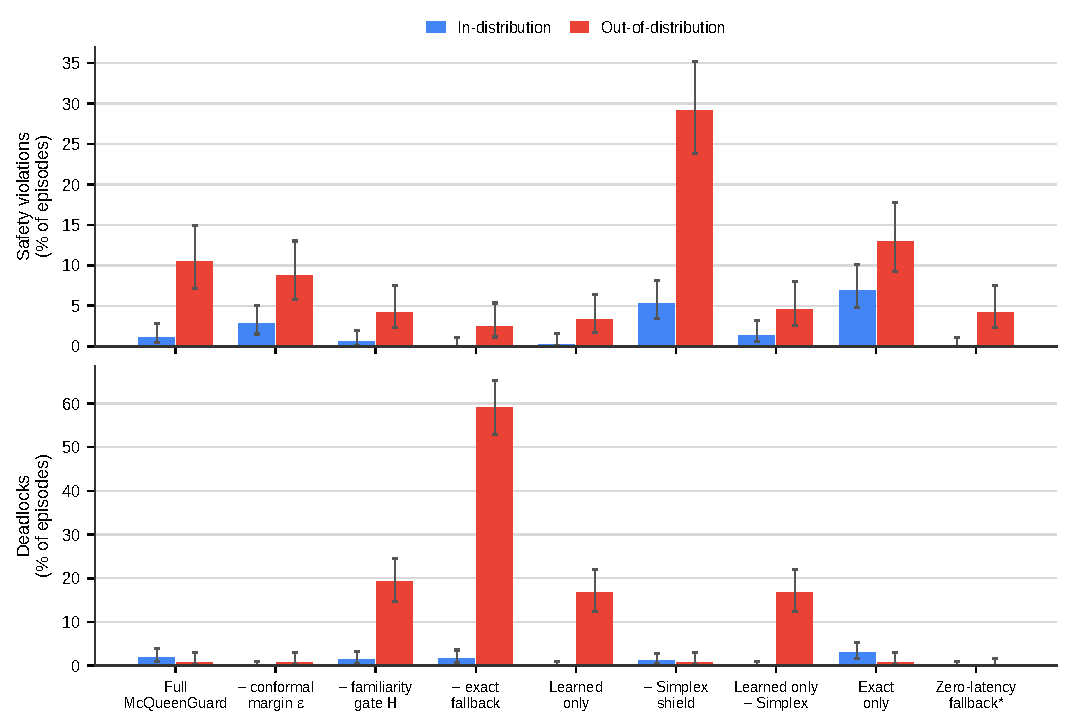
\includegraphics[width=\linewidth]{../figures/fig_r2_ablation.pdf}
\caption{Ablation: safety violations and deadlocks in the in-distribution and out-of-distribution categories (95\,\% Wilson intervals).}\label{fig:abl}
\end{figure}

\textbf{Findings of the ablation.}
\begin{itemize}[leftmargin=1.3em,itemsep=2pt]
\item \emph{Learned verifier.} Without it (exact verification only), 93\,\% of the decisions missed the 100\,ms decision period, and the safety-violation rate was 9.3\,\% against 4.8\,\% ($p<0.001$). The learned verifier is the component that makes runtime verification usable in the control loop.
\item \emph{Conformal margin.} Without the margin, the share of executed commands with verified risk $\ge\theta$ rose from 14.4\,\% to 21.4\,\% and collisions from 1.0\,\% to 1.5\,\%; the difference in safety violations (5.2\,\%, $p=0.88$) is within the statistical uncertainty of 600 episodes. The margin's main effect is on false admissions (Table~\ref{tab:pol}).
\item \emph{Familiarity check.} Without it, the learned verifier was also used in the high-noise and unseen-weather categories. This reduced exact fallbacks and the safety-violation rate (2.0\,\%), but the vehicle deadlocked in 8.5\,\% of the episodes: in the high-noise category the out-of-distribution estimates kept it at 5.4\,km/h on average and it did not clear the crosswalk in 68\,\% of the episodes. Evaluated on the decisions of the complete framework, removing the check would raise false admissions in the unseen-weather category from 0.00\,\% to 5.61\,\% of the decisions (Table~\ref{tab:ood}).
\item \emph{Exact fallback.} Replacing the exact fallback by the conservative fallback control gave the fewest safety violations (1.0\,\%) but 24.7\,\% deadlocks: 47\,\% of the decisions were conservative, and the vehicle did not clear the crosswalk in any high-noise or unseen-weather episode. The exact fallback is therefore what preserves progress when the learned verifier cannot be admitted.
\item \emph{Learned verifier without admission.} Using the learned verifier unconditionally gave 1.5\,\% safety violations with the Simplex shield and 2.7\,\% without it, but 6.7\,\% and 6.7\,\% deadlocks and no bound on false admissions (up to 28.60\,\% of the unseen-weather decisions).
\item \emph{Simplex shield.} Without the shield, the safety-violation rate rose to 14.8\,\% and collisions to 7.0\,\% ($p<0.001$). The shield covers the interval in which an exact result is pending.
\item \emph{Latency of the exact fallback.} With an idealised zero-latency fallback, the complete framework reached 1.7\,\% safety violations and 1.0\,\% collisions with 0.0\,\% deadlocks. The remaining gap of the deployable framework is therefore caused by the time spent in PRISM rather than by the admission logic.
\end{itemize}
No single component can be removed without losing liveness (more deadlocks), safety (more violations) or the bound on false admissions. The complete framework offers the best balance of these three properties among the deployable configurations; its remaining weakness is the latency of the exact fallback.

\textbf{Large-scale preservation analysis.} Table~2 illustrates decision preservation with twelve cases. To provide evidence at scale, every
third decision of the complete framework in all 600 episodes was additionally verified exactly for all five actions, outside the timed
decision path (25,466 decisions: 19,201 in-distribution and 6,265 out of
distribution). On this decision stream we evaluate four admission policies (Table~\ref{tab:pol}, Figure~\ref{fig:pres}a): no admission rule, the
conformal margin only, the familiarity check only, and both, as in McQueenGuard. A \emph{false admission} is a decision in which a learned result
is admitted although the exact unsafe probability of the admitted action is at least $\theta$; Corollary~1 bounds its probability by $\alpha=5\,\%$.
The counterfactual policies are evaluated on the states visited by the complete framework.

\begin{table}[h]
\centering\small
\caption{Admission policies on 25,466 exactly verified decisions. Admitted: share of decisions admitted to the learned verifier;
false admissions in \% of all decisions and of admitted decisions; agreement: admitted learned action equals the exact action.}\label{tab:pol}
\begin{adjustbox}{max width=\linewidth}
\begin{tabular}{lcccccccc}
\toprule
 & \multicolumn{4}{c}{In-distribution} & \multicolumn{4}{c}{Out-of-distribution} \\
\cmidrule(lr){2-5}\cmidrule(lr){6-9}
 & Admitted & \multicolumn{2}{c}{False admissions} & Agreement & Admitted & \multicolumn{2}{c}{False admissions} & Agreement \\
Admission policy & (\%) & (\% dec.) & (\% adm.) & (\%) & (\%) & (\% dec.) & (\% adm.) & (\%) \\
\midrule
No admission (learned verifier only) & 100.0 & 5.36 & 5.36 & 67.5 & 100.0 & 12.15 & 12.15 & 58.7 \\
Conformal margin only & 95.9 & 2.04 & 2.12 & 59.7 & 81.7 & 2.25 & 2.75 & 54.8 \\
Familiarity gate only & 96.9 & 3.54 & 3.65 & 67.4 & 57.3 & 1.44 & 2.51 & 68.1 \\
Margin + gate (McQueenGuard) & 95.4 & 1.99 & 2.09 & 59.7 & 56.7 & 0.77 & 1.35 & 63.3 \\
\bottomrule
\end{tabular}
\end{adjustbox}
\end{table}

\begin{table}[h]
\centering\small
\caption{Decision preservation (Theorem~1) on the 21,881 admitted decisions. $\varepsilon_U=0.101$ is the
split-conformal bound on $\max_a|U(a)-\hat U(a)|$ ($\alpha=0.05$) and $m(x)=\mathcal{T}(k)-2\varepsilon_U$. Regret: mean exact utility loss of
the disagreeing decisions.}\label{tab:th1}
\begin{adjustbox}{max width=\linewidth}
\begin{tabular}{lcccc}
\toprule
Group of admitted decisions & Decisions & Agreement (\%) & Regret & Unsafe admitted actions \\
\midrule
Calibrated condition $m(x)>0$ & 0 & -- & -- & 0 \\
Realised utility error satisfies $2\max_a|U(a)-\hat U(a)|<\mathcal{T}(k)$ & 690 & 100.0 & -- & 0 \\
Realised utility error does not satisfy the condition & 17,484 & 70.1 & 0.009 & 0 \\
Single admissible action & 32 & 100.0 & -- & 0 \\
Different learned and exact admissible sets & 3,675 & 5.9 & 0.027 & 431 \\
\bottomrule
\end{tabular}
\end{adjustbox}
\end{table}

\begin{figure}[h]
\centering
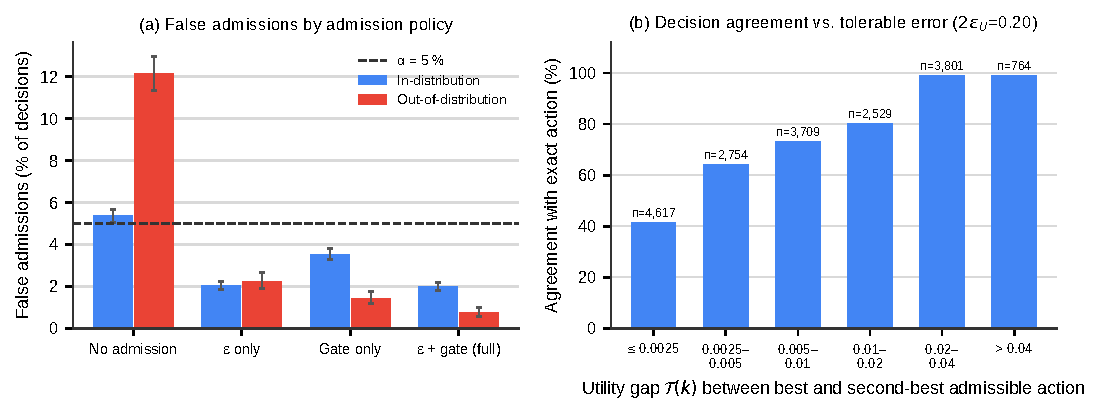
\includegraphics[width=\linewidth]{../figures/fig_r2_preservation.pdf}
\caption{(a) False admissions per decision for four admission policies (95\,\% Wilson intervals). (b) Agreement between the admitted learned
action and the exact action as a function of the utility gap $\mathcal{T}(k)$ (admitted decisions with the same learned and exact admissible set);
the calibrated condition of Theorem~1 requires $\mathcal{T}(k)>2\varepsilon_U$.}\label{fig:pres}
\end{figure}

\textbf{Findings of the preservation analysis.}
\begin{itemize}[leftmargin=1.3em,itemsep=2pt]
\item \emph{Safety preservation.} With McQueenGuard's admission rule, false admissions occurred in 1.99\,\% of the in-distribution and 0.77\,\% of the out-of-distribution decisions, below $\alpha=5\,\%$ as stated by Corollary~1; without an admission rule the rates were 5.36\,\% and 12.15\,\%. On risk-relevant decisions the rates were 4.24\,\% of the decisions with the rule and 17.63\,\% without it; per admitted risk-relevant decision the rate with the rule was 5.51\,\%, slightly above $\alpha$, which again reflects that the guarantee of Corollary~1 is marginal rather than conditional. The margin contributes most in-distribution (3.54\,\% with the familiarity check alone), the familiarity check out of distribution (2.25\,\% with the margin alone).
\item \emph{Decision preservation.} The admitted learned action equalled the exact action in 60.3\,\% of the 21,881 admitted decisions. The disagreements are mostly harmless: in 96\,\% of them the learned action was safe and in 69\,\% it was more cautious than the exact action; within the same admissible set the mean utility loss was 0.009.
\item \emph{Theorem~1 at scale.} Whenever the realised utility error satisfied the condition of Theorem~1, the decisions agreed in 100.0\,\% of the 690 cases, as the theorem predicts (a consistency check of the statement and of our implementation). With the calibrated utility bound $\varepsilon_U=0.101$, however, the condition $m(x)>0$ was not satisfied by any decision, because the utility gap $\mathcal{T}(k)$ between the best and second-best admissible actions is small in this scenario (median 0.007, 90th percentile 0.030). Theorem~1 is a sufficient condition and is conservative when candidate actions have similar utilities. All 431 unsafe admissions occurred in decisions whose learned and exact admissible sets differed, that is, when the probability bound failed for one of the actions; this is the event bounded by Corollary~1.
\end{itemize}
These results support the safety-preservation result at scale and qualify the decision-preservation result: the framework guarantees, under the calibration assumptions, that admitted actions are safe with probability at least $1-\alpha$, but it does not guarantee that the learned and exact verification select the same action. We have revised the text of Sections~5.1 and 6.5 accordingly.

%-----------------------------------------------------------------------------------------------------
\clearpage
\section*{6.11 \quad Reliability of the Error Bound under Out-of-Distribution Conditions and Latency Breakdown}
\addcontentsline{toc}{section}{6.11 Out-of-distribution reliability and latency breakdown}
\textbf{Error-bound reliability.} Table~\ref{tab:ood} and Figure~\ref{fig:ood} report, for each scenario category, the coverage of the calibrated
margin, the false-admission rate and the fallback rate on the exactly verified decisions of the complete framework, together with the
closed-loop safety outcomes. Coverage is reported for all decisions, for the \emph{risk-relevant} decisions (at least one candidate action with
exact unsafe probability $\ge 10^{-3}$) and for the admitted decisions. The sensor-noise shift study of Section~6.12 complements this analysis
with a gradual shift of the noise distribution.

\begin{table}[h]
\centering\small
\caption{Error-bound coverage, admission and safety outcomes per scenario category (complete framework). The four categories below the line are
out of distribution. False admissions in \% of decisions; ``w/o $\mathcal{H}$'': counterfactual without the familiarity check.}\label{tab:ood}
\begin{adjustbox}{max width=\linewidth}
\begin{tabular}{lcccccccccc}
\toprule
 & Labelled & Familiar & Fallback & \multicolumn{3}{c}{Coverage of $\varepsilon$ (\%)} & \multicolumn{2}{c}{False admissions (\%)} & \multicolumn{2}{c}{Episodes (\%)} \\
\cmidrule(lr){5-7}\cmidrule(lr){8-9}\cmidrule(lr){10-11}
Category & decisions & (\%) & all / risk-rel. & all & risk-relevant & admitted & McQueenGuard & w/o $\mathcal{H}$ & collision & safety viol. \\
\midrule
Clear (10--30) & 3,936 & 98.6 & 2.5 / 7.0 & 96.1 & 87.6 & 96.3 & 1.96 & 2.08 & 0.0 & 0.0 \\
Clear (35--50) & 2,465 & 97.8 & 4.9 / 9.5 & 95.1 & 88.8 & 95.2 & 1.87 & 1.95 & 0.0 & 3.3 \\
Fog (10--30) & 4,281 & 99.9 & 2.9 / 8.6 & 96.9 & 90.7 & 97.0 & 1.49 & 1.49 & 0.0 & 0.0 \\
Fog (35--50) & 2,350 & 98.3 & 7.5 / 17.5 & 96.3 & 90.7 & 97.0 & 1.79 & 1.79 & 0.0 & 1.7 \\
Rain (10--30) & 4,017 & 100.0 & 3.6 / 8.5 & 94.5 & 86.8 & 94.6 & 3.34 & 3.34 & 0.0 & 0.0 \\
Rain (35--50) & 2,152 & 97.3 & 9.9 / 17.8 & 96.6 & 93.0 & 97.1 & 0.93 & 0.98 & 0.0 & 1.7 \\
\midrule
High speed (50--60) & 1,285 & 84.0 & 21.0 / 29.3 & 94.8 & 90.8 & 95.7 & 2.18 & 2.80 & 3.3 & 10.0 \\
Novel trajectory & 2,642 & 98.5 & 3.9 / 8.3 & 97.9 & 92.9 & 98.1 & 0.76 & 0.83 & 6.7 & 18.3 \\
High noise & 1,055 & 0.0 & 100.0 / 100.0 & 97.6 & 94.9 & -- & 0.00 & 1.04 & 0.0 & 6.7 \\
Unseen weather & 1,283 & 0.0 & 100.0 / 100.0 & 89.6 & 82.2 & -- & 0.00 & 5.61 & 0.0 & 6.7 \\
\bottomrule
\end{tabular}
\end{adjustbox}
\end{table}

\begin{figure}[h]
\centering
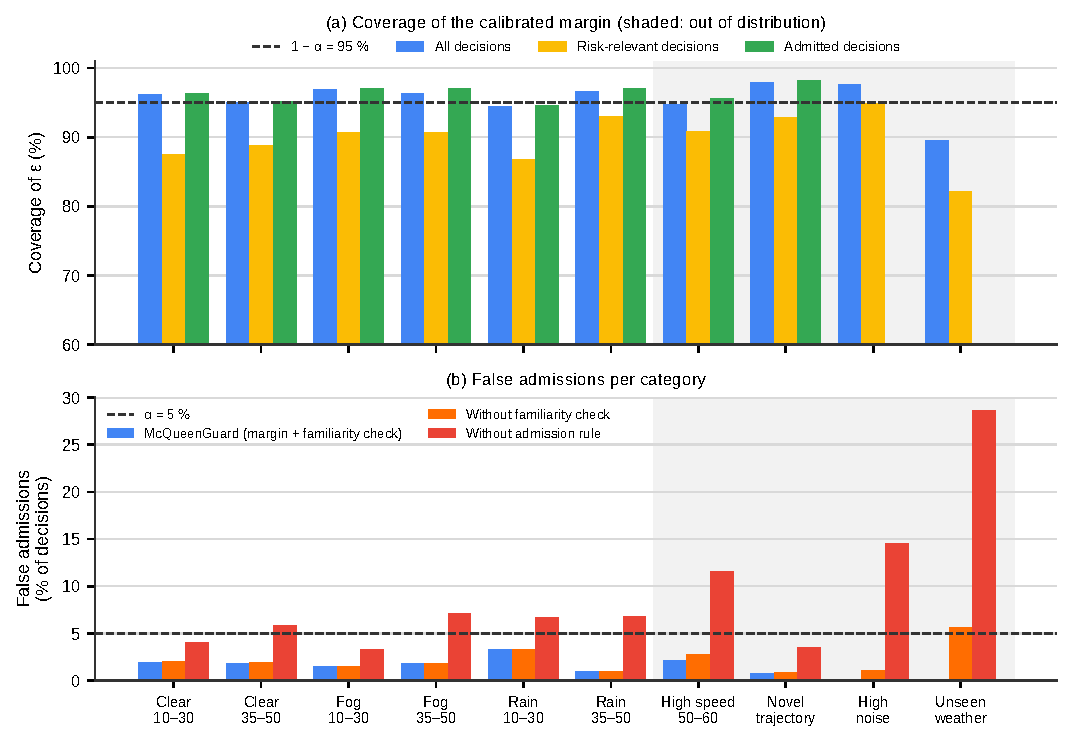
\includegraphics[width=\linewidth]{../figures/fig_r2_ood.pdf}
\caption{(a) Coverage of the calibrated margin per category. (b) False admissions per category for McQueenGuard and for two counterfactual
admission rules evaluated on the same decisions. Shaded: out-of-distribution categories.}\label{fig:ood}
\end{figure}

\textbf{Findings.}
\begin{itemize}[leftmargin=1.3em,itemsep=2pt]
\item \emph{In-distribution.} The coverage of the margin over all decisions was 94.5--96.9\,\%, close to the nominal 95\,\%, and false admissions stayed at or below 3.34\,\% of the decisions. On risk-relevant decisions coverage was lower (86.8--93.0\,\%): the conformal guarantee of Equation~(26) is marginal over the calibration distribution and does not hold conditionally on a subset of difficult decisions. Fallback rates were 2.5--9.9\,\% of the decisions.
\item \emph{High speed.} 16.0\,\% of the decisions were outside $\mathcal{H}$, the fallback rate rose to 21.0\,\%, coverage stayed at 94.8\,\% and false admissions at 2.18\,\%. With an idealised zero-latency fallback no safety violation occurred in this category (0.0\,\% against 10.0\,\%, exact McNemar $p=0.031$), so these violations are attributable to the time spent waiting for PRISM.
\item \emph{High noise and unseen weather.} The familiarity check rejected every decision (fallback rate 100\,\%), so the learned verifier was not used. This was necessary: under unseen weather, coverage fell to 89.6\,\% (82.2\,\% on risk-relevant decisions), and false admissions would have reached 5.61\,\% of the decisions without the check and 28.60\,\% without any admission rule. The 6.7\,\% and 6.7\,\% safety violations in these categories (4 and 4 episodes) did not occur with the idealised zero-latency fallback, which points to exact-verification latency as their cause; with 60 episodes per category this is indicative only.
\item \emph{Novel trajectories.} Running and occluded pedestrians did not change the feature distribution enough to be detected (98.5\,\% familiar), and the margin remained valid (97.9\,\% coverage, 0.76\,\% false admissions). Nevertheless, this category had the highest safety-violation rate of the complete framework (18.3\,\%, 6.7\,\% collisions); exact verification only reached 18.3\,\% and the zero-latency variant 16.7\,\%, and all baselines had 15.0--25.0\,\%. The error bound is defined with respect to the exact verification result, so it cannot detect behaviour that the verification model itself does not represent.
\item \emph{Familiarity check as a detector.} The check detects shifts of the input distribution, but its Mahalanobis score is a weak predictor of individual bound failures (area under the ROC curve 0.56; coverage 96.1\,\% on familiar and 93.0\,\% on unfamiliar decisions). Familiarity alone does not certify the bound; the online recalibration of Section~6.12 addresses this for gradual shifts.
\end{itemize}
The empirical coverage of 97.8\,\% in Table~4 should therefore be read as an in-distribution result. Out of distribution, the framework does not rely on the bound remaining valid: it relies on detecting the shift and falling back to exact verification, which worked for sensor-noise and weather shifts, and it cannot protect against modelling gaps such as unmodelled pedestrian behaviour.

\textbf{Relation to Table~3.} The fallback rates of Table~\ref{tab:ood} are not directly comparable with those of Table~3. Table~3 counts the
verification mode at the critical decision point of each CARLA scenario run, whereas Table~\ref{tab:ood} counts every decision of an episode,
most of which are routine decisions far from the pedestrian. On risk-relevant decisions, which are closer to the critical decision points, the
testbed fallback rates follow the ordering of Table~3 (clear $<$ fog $<$ rain, higher at higher speed, and 100\,\% under high noise and unseen
weather) at lower absolute values. The exception is the novel-trajectory category (8.3\,\% here against 87\,\% in Table~3):
in the testbed, running and occluded pedestrians produce feature values inside the training range, so the familiarity check does not flag them.
This difference indicates that familiarity must be defined on features that capture pedestrian behaviour if novel trajectories are to be routed to
exact verification; as shown above, exact verification would not remove the resulting violations, because they originate in the verification model.

\textbf{Latency breakdown.} Table~\ref{tab:lat} decomposes the decision latency. The runtime rows of Table~4 (2.1\,ms against 148.6\,ms, about
70$\times$) compare the inference time of the learned verifier with the time of one exact verification; they are component times, not the
end-to-end overhead. In the revised Table~4 these rows are labelled ``Learned-verifier inference time'' and ``Exact PRISM verification time per
decision'', and the end-to-end values of Table~\ref{tab:lat} are added.

\begin{table}[h]
\centering\small
\caption{Decomposition of the decision latency (single CPU thread; exact path measured on 600 runtime queries with a warm
PRISM server).}\label{tab:lat}
\begin{tabular}{lcc}
\toprule
Component & mean & p99 \\
\midrule
\multicolumn{3}{l}{\textit{Learned path (per decision)}} \\
Feature extraction $\phi(x)$ & 3.9\,$\mu$s & 9.1\,$\mu$s \\
MLP inference, NumPy (FP64) & 12.9\,$\mu$s & 32.0\,$\mu$s \\
MLP inference, ONNX Runtime (FP32) & 8.3\,$\mu$s & 22.2\,$\mu$s \\
Familiarity gate ($x\in\mathcal{H}$) & 8.2\,$\mu$s & 22.2\,$\mu$s \\
Admission test and lexicographic selection & 2.6\,$\mu$s & 5.4\,$\mu$s \\
\textbf{Complete learned decision} (with NumPy inference) & \textbf{43.6\,$\mu$s} & \textbf{94.6\,$\mu$s} \\
\midrule\multicolumn{3}{l}{\textit{Exact path (per fallback, PRISM 4.8.1 warm server)}} \\
Valuation $\lambda$ and pMDP instantiation (model generation) & 49.1\,$\mu$s & -- \\
Model file transfer and inter-process communication (excluding generation) & 1.4\,ms & -- \\
PRISM model parsing & 3.4\,ms & 8\,ms \\
PRISM model construction and model checking & 387\,ms & 2,244\,ms \\
\textbf{Complete exact verification} & \textbf{392\,ms} & \textbf{2,248\,ms} \\
\midrule\multicolumn{3}{l}{\textit{End-to-end decision latency in closed loop (all decisions of the 600 episodes)}} \\
McQueenGuard (learned decisions and exact fallbacks) & 49.1\,ms & 794\,ms \\
Exact verification at every decision & 334\,ms & 1,525\,ms \\
\bottomrule
\end{tabular}
\end{table}

The learned path is dominated by MLP inference in the NumPy implementation used in the control loop (12.9\,$\mu$s) and by the familiarity check (8.2\,$\mu$s); with ONNX Runtime, inference takes 8.3\,$\mu$s. Exact verification is dominated by model construction and model checking inside PRISM (99\,\% of its time). The ratio between one exact verification and one learned decision is about 9,000$\times$ (about 47,000$\times$ for inference alone), but because 14\,\% of the decisions fall back to exact verification, the end-to-end mean decision latency falls only from 334\,ms to 49.1\,ms (6.8$\times$, an 85\,\% reduction), and the 99th percentile (794\,ms) is set by the fallbacks. Perception (90--150\,ms) and actuation (0.1\,s delay) latencies are the same for all methods and are not included. Measured in time rather than in decisions, exact verification is not a minor share: the 14\,\% exact decisions occupy 36\,\% of the driving time, because each one blocks the planner until it completes.

%-----------------------------------------------------------------------------------------------------
\clearpage
\section*{6.12 \quad Embedded Deployment and Sensor-Noise Shift}
\addcontentsline{toc}{section}{6.12 Embedded deployment and sensor-noise shift}
\textbf{Latency, memory and energy of the learned verifier.} The learned verifier was exported to ONNX and measured in four runtimes with one
thread and batch size one (20,000 inferences each; 10,000 for PyTorch); the complete learned decision path was measured on 3,000 recorded runtime observations
from all ten categories (Table~\ref{tab:emb}; the same measurements are decomposed in Table~\ref{tab:lat}). The MLP has 7,786 parameters and needs 7,616 multiply-accumulate operations per
inference.

\begin{table}[h]
\centering\small
\caption{Measured latency of the learned and exact verification paths (single CPU thread). The NumPy, ONNX FP32, learned-path and PRISM rows are the
measurements of Table~\ref{tab:lat}; the PyTorch and INT8 rows come from a separate benchmark run on the same machine.}\label{tab:emb}
\begin{tabular}{lcc}
\toprule
Component & mean & p99 \\
\midrule
MLP inference only, NumPy (FP64) & 12.9\,$\mu$s & 32.0\,$\mu$s \\
MLP inference only, PyTorch eager (FP32) & 49.2\,$\mu$s & 117.3\,$\mu$s \\
MLP inference only, ONNX Runtime (FP32) & 8.3\,$\mu$s & 22.2\,$\mu$s \\
MLP inference only, ONNX Runtime (INT8) & 14.1\,$\mu$s & 39.0\,$\mu$s \\
Complete learned decision (features, MLP, familiarity check, admission, action) & 43.6\,$\mu$s & 94.6\,$\mu$s \\
Exact verification, PRISM 4.8.1 warm server (sparse engine) & 392\,ms & 2,248\,ms \\
\bottomrule
\end{tabular}
\end{table}

\emph{Memory.} The weights occupy 30.4\,KiB in FP32 (ONNX file 31.8\,KiB; INT8 file
13.7\,KiB) and the activations 680\,bytes. A minimal Python process with ONNX Runtime serving
the INT8 model has a resident set of 54\,MB, of which the inference session accounts for
9\,MB; the PRISM verification server (Java virtual machine) reaches 251\,MB.
Dynamic INT8 quantisation changes the predictions by at most 0.094 (MAE
0.0153 for FP32 and 0.0144 for INT8); after recalibration the INT8 margin is
0.027 with 95.0\,\% coverage, so the admission mechanism remains valid with a
wider margin. On this x86 CPU the INT8 model is not faster than FP32; its benefit is the smaller model.

\emph{Projection to NVIDIA Jetson AGX Orin.} No Orin board was available. Table~\ref{tab:orin} therefore projects the measured latencies to the Orin
CPU (twelve Arm Cortex-A78AE cores at up to 2.2\,GHz, module power 15--60\,W) with an explicit single-thread slow-down band of 1.5--4$\times$, and
bounds the energy per decision by the module power envelope multiplied by the decision time. This bound is conservative, because the module power
includes idle subsystems.

\begin{table}[h]
\centering\small
\caption{Projected decision latency and energy per decision on Jetson AGX Orin (assumption-based, see text).}\label{tab:orin}
\begin{adjustbox}{max width=\linewidth}
\begin{tabular}{lcccccc}
\toprule
Slow-down & \multicolumn{2}{c}{Learned decision} & \multicolumn{2}{c}{Exact verification} & \multicolumn{2}{c}{Energy per decision, 15\,W / 60\,W (upper bound)} \\
\cmidrule(lr){2-3}\cmidrule(lr){4-5}\cmidrule(lr){6-7}
assumption & mean & p99 & mean & p99 & learned & exact \\
\midrule
Low ($\times$1.5) & 65\,$\mu$s & 142\,$\mu$s & 588\,ms & 3,371\,ms & 1.0 / 3.9\,mJ & 8.8 / 35.3\,J \\
Central ($\times$2.5) & 109\,$\mu$s & 237\,$\mu$s & 980\,ms & 5,619\,ms & 1.6 / 6.5\,mJ & 14.7 / 58.8\,J \\
High ($\times$4.0) & 174\,$\mu$s & 379\,$\mu$s & 1,568\,ms & 8,990\,ms & 2.6 / 10.5\,mJ & 23.5 / 94.1\,J \\
\bottomrule
\end{tabular}
\end{adjustbox}
\end{table}

\textbf{Closed loop under embedded timing.} To test whether the safety results survive slower hardware, 100 episodes (10 per category, the same
instances as in Section~6.9) were re-run with every measured computation time multiplied by 2.5, the central projection (Table~\ref{tab:et},
Figure~\ref{fig:et}).

\begin{table}[h]
\centering\small
\caption{Testbed timing and embedded timing ($\times$2.5), 100 paired episodes per method.}\label{tab:et}
\begin{adjustbox}{max width=\linewidth}
\begin{tabular}{lcccccc}
\toprule
 & \multicolumn{3}{c}{Testbed timing} & \multicolumn{3}{c}{Embedded timing ($\times$2.5)} \\
\cmidrule(lr){2-4}\cmidrule(lr){5-7}
Method & latency (ms) & misses (\%) & safety viol. (\%) & latency (ms) & misses (\%) & safety viol. (\%) \\
\midrule
McQueenGuard & 51 & 13.5 & 5.0 & 68 & 7.9 & 7.0 \\
McQueenGuard (exact only) & 337 & 92.1 & 9.0 & 820 & 100.0 & 15.0 \\
VerifAI RA & 0.06 & 0.0 & 3.0 & 0.24 & 0.0 & 3.0 \\
MPC & 17 & 0.2 & 11.0 & 31 & 1.9 & 9.0 \\
Rule-based (IDM+AEB) & $<$0.01 & 0.0 & 4.0 & $<$0.01 & 0.0 & 4.0 \\
End-to-end RL (PPO) & 0.04 & 0.0 & 8.0 & 0.16 & 0.0 & 8.0 \\
\bottomrule
\end{tabular}
\end{adjustbox}
\end{table}
\begin{figure}[h]
\centering
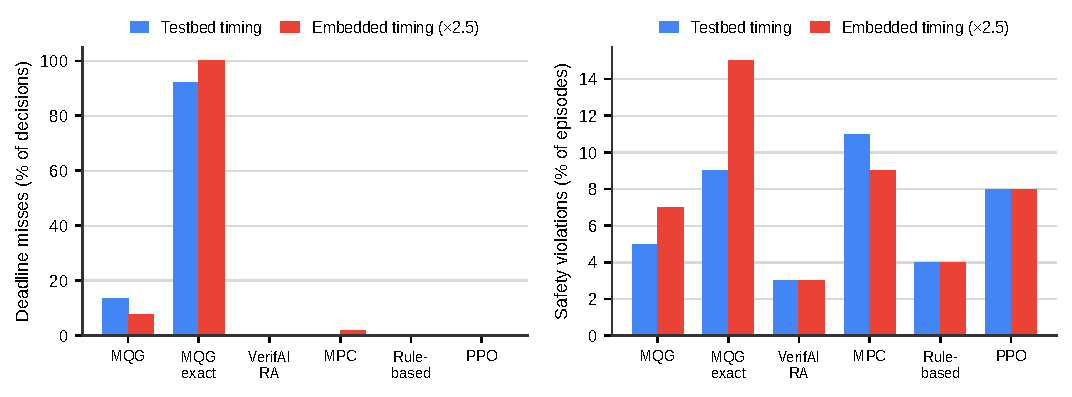
\includegraphics[width=0.95\linewidth]{../figures/fig_c6_embedded_timing.pdf}
\caption{Deadline misses and safety violations with testbed timing and embedded timing (MQG = McQueenGuard).}\label{fig:et}
\end{figure}

\textbf{Findings.} Methods whose decisions take well under 100\,ms (VerifAI, the rule-based planner and PPO) were not affected. MPC stayed below the decision period on average. McQueenGuard's safety violations rose from 5\,\% to 7\,\% and those of exact verification only from 9\,\% to 15\,\%, because each fallback waits 2.5 times longer for PRISM. The learned path itself remains far below the decision period on embedded hardware; the exact fallback is the bottleneck. On a vehicle, the exact verifier should run on a dedicated core with a bounded model size or be replaced by a faster exact engine, while the fallback safety control covers the waiting time. McQueenGuard's share of missed deadlines fell under the slower timing because each exact verification blocks the planner for longer, so fewer decisions are taken during fallback periods. With 100 episodes per method these differences are indicative rather than statistically conclusive.

\textbf{Shift of the sensor-noise distribution (simulation to real).} At test time the perception noise model was replaced by a combined shift of
severity $s\in\{0,0.5,1\}$ that the framework is not told about: Student-$t$ noise with $6-4s$ degrees of freedom and a scale of $1+1.5s$, a
systematic lateral bias of $0.6s$\,m, $25s$\,\% additional drop-outs and $120s$\,ms additional latency. Three mechanisms act under such a shift:
(i) the familiarity check routes unfamiliar feature vectors to exact verification; (ii) the exact results of these fallbacks, together with
shadow audits of 10\,\% of the admitted decisions run outside the critical path, are used to recompute the conformal quantile of Equation~(25)
over a rolling window of the last 200 residuals, without letting $\varepsilon$ fall below its offline value (Algorithm~1, lines~27--28);
(iii) the Simplex shield and the exact fallback remain active regardless of the learned verifier. Table~\ref{tab:ss} and Figure~\ref{fig:ss}
evaluate the admission policies on exactly verified decisions collected under the shift, and Table~\ref{tab:sc} reports the closed-loop outcomes.

\begin{table}[h]
\centering\small
\caption{Decision-stream analysis under the sensor-noise shift. Admission rate / unsafe-admission rate (\% of admitted decisions).}\label{tab:ss}
\begin{adjustbox}{max width=\linewidth}
\begin{tabular}{cccccccc}
\toprule
 & Verified & Coverage of & Familiar & Static margin, & Static margin & + online & $\varepsilon$ after \\
$s$ & decisions & static margin (\%) & (\%) & no check & + check & recalibration & recalibration \\
\midrule
0.0 & 1,166 & 95.4 & 99.3 & 87.7 / 2.2 & 87.2 / 2.2 & 85.2 / 1.1 & 0.020 \\
0.5 & 1,125 & 92.9 & 97.8 & 91.4 / 3.4 & 89.5 / 3.3 & 71.4 / 1.5 & 0.040 \\
1.0 & 1,162 & 94.1 & 88.4 & 88.0 / 3.8 & 78.8 / 3.8 & 67.4 / 1.8 & 0.033 \\
\bottomrule
\end{tabular}
\end{adjustbox}
\end{table}
\begin{figure}[h]
\centering
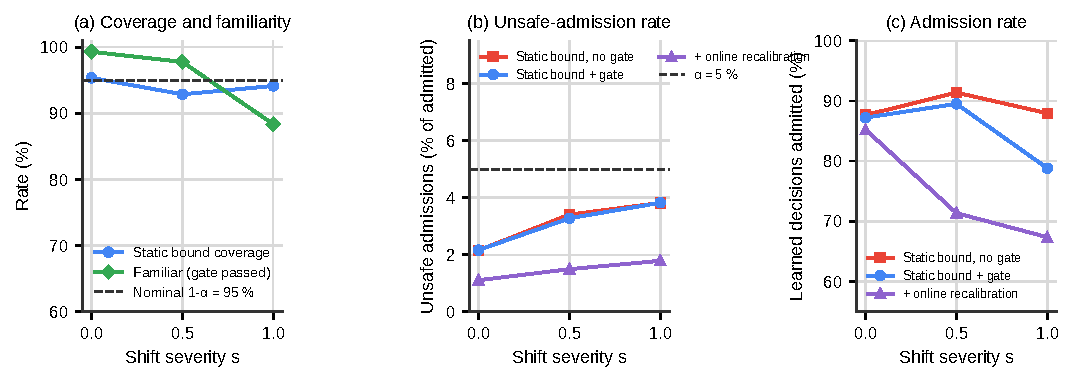
\includegraphics[width=\linewidth]{../figures/fig_c6_shift_stream.pdf}
\caption{Effect of the sensor-noise shift on (a) coverage and familiarity, (b) unsafe-admission rate and (c) admission rate.}\label{fig:ss}
\end{figure}
\begin{table}[h]
\centering\small
\caption{Closed loop under the sensor-noise shift: collision / safety-violation rate (\%), 30 episodes per severity and method
(in-distribution categories).}\label{tab:sc}
\begin{tabular}{lccc}
\toprule
Method & $s=0.0$ & $s=0.5$ & $s=1.0$ \\
\midrule
McQueenGuard (static bound) & 0.0 / 0.0 & 0.0 / 0.0 & 0.0 / 0.0 \\
McQueenGuard (online recalibration) & 0.0 / 3.3 & 0.0 / 6.7 & 0.0 / 0.0 \\
VerifAI RA & 0.0 / 0.0 & 3.3 / 13.3 & 0.0 / 20.0 \\
MPC & 0.0 / 3.3 & 0.0 / 0.0 & 3.3 / 10.0 \\
Rule-based (IDM+AEB) & 0.0 / 0.0 & 0.0 / 0.0 & 0.0 / 3.3 \\
End-to-end RL (PPO) & 0.0 / 3.3 & 0.0 / 10.0 & 3.3 / 10.0 \\
\bottomrule
\end{tabular}
\end{table}

\textbf{Findings.} The coverage of the offline margin varied between 92.9 and 95.4\,\% (94.1\,\% at $s=1$), and the unsafe-admission rate of the static margin rose from 2.2\,\% to 3.8\,\% of the admitted decisions. The familiarity check removed 12\,\% of the shifted decisions at $s=1$. With online recalibration, $\varepsilon$ grew to 0.033 and the unsafe-admission rate remained between 1.1 and 1.8\,\% across the severities, at the price of admitting 67\,\% instead of 79\,\% of the decisions. The guarantee thus degrades gradually and the framework trades speed-up for assurance automatically. Recalibration does not restore exchangeability, so under a persistent shift the statistical statement remains conditional on the recalibration window. In closed loop (Table~\ref{tab:sc}) neither McQueenGuard configuration had a collision at any severity, whereas VerifAI, MPC and PPO reached 20\,\%, 10\,\% and 10\,\% safety violations at $s=1$. The configuration with online recalibration had slightly more safety violations than the static one at $s=0$ and $s=0.5$, consistent with its higher fallback rate; with 30 episodes per cell, differences of one or two episodes are not significant.

%-----------------------------------------------------------------------------------------------------
\section*{Revisions of existing text in Sections 5 and 6}
\addcontentsline{toc}{section}{Revisions of existing text in Sections 5 and 6}
\begin{itemize}[leftmargin=1.3em,itemsep=2pt]
\item \emph{Section~5.1, after the proof of Theorem~1}: ``Theorem~1 gives a sufficient condition. When candidate actions have similar utilities, the tolerable error $\mathcal{T}(k)$ is small and the condition $2\varepsilon_{\Gamma'}(x)<\mathcal{T}(k)$ is rarely met with a calibrated bound; the learned and exact verification may then select different actions. Safety is not affected by such deviations as long as the admitted action satisfies the conservative safety condition of Theorem~2 (see Section~6.10).''
\item \emph{Section~6.5, after the discussion of Table~2}: ``Table~2 illustrates the decision-preservation condition on selected cases. A large-scale evaluation over 25,466 exactly verified decisions is reported in Section~6.10.''
\item \emph{Table~4, runtime rows}: ``Inference time (learned verifier)'' becomes ``Learned-verifier inference time''; ``Exact PRISM verification time'' becomes ``Exact PRISM verification time per decision''; ``Speedup factor'' becomes ``Speed-up of a single verification (inference only)''; and a footnote is added: ``Component times; the end-to-end decision latency in closed loop is reported in Table~\ref{tab:lat}.''
\end{itemize}

\section*{6.13 \quad Threats to Validity (additions to the former Section~6.8)}
\addcontentsline{toc}{section}{6.13 Threats to validity (additions)}
The following paragraph is added to the threats to validity:
\begin{quote}
The comparative, ablation and out-of-distribution results of Sections~6.9--6.12 were obtained in a closed-loop testbed that re-implements the pedestrian-crossing scenario with the sensing, weather and actuation characteristics of the CARLA configuration, rather than in CARLA itself; absolute rates are therefore not interchangeable with those of Sections~6.2--6.7. The baselines were implemented by the authors following the cited work; VerifAI's sampler and specification-monitor classes were used directly, and the PPO planner was trained for this scenario only. The embedded figures for NVIDIA Orin are projections from single-thread measurements under a stated slow-down band, and the energy figures are upper bounds derived from the module power envelope; no measurement on automotive hardware was performed. The error bound is defined with respect to the exact verification result; behaviour that the verification model does not represent, such as running or occluded pedestrians, is not covered by the bound and was the largest single source of safety violations of the complete framework and of exact verification only. Finally, the latency of exact verification is the main residual risk of the framework in closed loop; it is mitigated, but not removed, by the fallback safety control and the Simplex shield. The online recalibration of Section~6.12 does not restore exchangeability, so under a persistent distribution shift the statistical guarantee remains conditional on the recalibration window. Validation on automotive hardware and on a test vehicle is left to future work.
\end{quote}

\end{document}
